86. $f(x)=\cfrac{1-|x-2|}{x}=\begin{cases} \cfrac{1+x-2}{x},\ x\leqslant 2,\\ \cfrac{1-x+2}{x},\ x > 2.\end{cases}=\begin{cases} 1-\cfrac{1}{x},\ x\leqslant 2,\\ \cfrac{3}{x}-1,\ x > 2.\end{cases}$
$$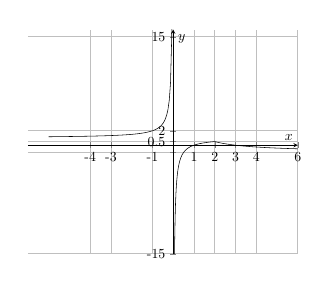
\begin{tikzpicture}[scale=0.5]
\begin{axis}[
    axis lines = middle,
    grid=major,
    legend pos={south west},
    xlabel = {$x$},
    %xlabel style={below right},
    ylabel = {$y$},
    ymin=-15,
    ymax=16,
    xmin=-7,
    xmax=6,
    xtick={-4,-3,-1,1,2,3,4,6},
    xticklabels={-4,-3,-1,1,2,3,4,6},
    ytick={-15,-1,0.5,2,15},
    yticklabels={-15, $ $,0.5,2,15},
                  ]
    \addplot[domain=-6:-0.01, samples=100, color=black] {1-(1/x)};
	\addplot[domain=0.01:2, samples=100, color=black] {1-(1/x)};
    \addplot[domain=2:6, samples=100, color=black] {-1+(3/x)};
    %\addplot[domain=2.01:6, samples=100, color=black] {2/(2-x)};
   % \addplot[domain=-3:3, samples=100, color=black] {-x};
     %\addlegendentry{$\text{Рис. 1}$};
\end{axis}
\end{tikzpicture}$$
По графику определим ответ $x\in(-\infty;-1]\cup(0;+\infty).$\\
